\documentclass[journal]{IEEEtran}

\usepackage{cite}
\usepackage{amsmath,amssymb}
\usepackage{graphicx}
\usepackage{tabularx}
\usepackage{array}
\usepackage{multirow}
\usepackage{makecell}
\usepackage{colortbl}
\usepackage{xcolor}
\usepackage{url}
\usepackage{xurl}
\usepackage{microtype}
\usepackage{balance}
\usepackage{enumitem}
\usepackage{siunitx}
\usepackage{xspace}
\usepackage[hidelinks]{hyperref}
\usepackage{orcidlink}
\usepackage{stfloats}
\usepackage[caption=false,font=footnotesize]{subfig}

\definecolor{TableHeader}{HTML}{E8EEF5}
\definecolor{TableBorder}{HTML}{3C536B}
\definecolor{AccentBlue}{HTML}{173F6B}
\arrayrulecolor{TableBorder}
\setlength{\arrayrulewidth}{0.48pt}
\setlength{\tabcolsep}{3.3pt}
\renewcommand{\arraystretch}{1.16}
\newcolumntype{Y}{>{\raggedright\arraybackslash}X}
\newcolumntype{C}{>{\centering\arraybackslash}X}
\newcommand{\THead}[1]{\cellcolor{TableHeader}\textbf{#1}}
\newcommand{\system}{\textsc{Africa-ZT-Edu}\xspace}

\hypersetup{
  pdftitle={AFRICA-ZT-EDU: A Policy-Centric Zero-Trust and Privacy-Preserving Architecture for Cross-Border Digital Education in Africa},
  pdfauthor={Abdessamad Bourkibate},
  pdfsubject={Zero trust, privacy engineering, digital education, Africa, verifiable credentials, cross-border data flows},
  pdfkeywords={zero trust, digital education, Africa, privacy engineering, verifiable credentials, differential privacy, federated analytics}
}
\Urlmuskip=0mu plus 1mu
\setlist[itemize]{leftmargin=*,nosep}
\setlist[enumerate]{leftmargin=*,nosep}
\sisetup{round-mode=places,round-precision=4}

\newcommand{\papercutoff}{18 August 2026}
\newcommand{\scorezero}{0}
\newcommand{\scorehalf}{0.5}
\newcommand{\scorefull}{1}

\title{AFRICA-ZT-EDU: A Policy-Centric Zero-Trust and Privacy-Preserving Architecture for Cross-Border Digital Education in Africa}

\author{Abdessamad Bourkibate\,\orcidlink{0009-0000-6186-8071}\\[-0.2ex]
{\small Department of Computer Science, University of the People, Pasadena, CA, USA.}\\[-0.15ex]
{\small Faculty of Legal, Economic and Social Sciences, Cadi Ayyad University, Marrakech, Morocco.}\\[-0.15ex]
{\small Share In, Casablanca, Morocco.}\\[-0.15ex]
{\small ORCID: \href{https://orcid.org/0009-0000-6186-8071}{0009-0000-6186-8071}.}}


\markboth{Original Research Article -- Digital Education, Privacy \& Cybersecurity -- August 2026}{Bourkibate: AFRICA-ZT-EDU}

\begin{document}
\maketitle
\begin{center}
\begin{minipage}{0.34\textwidth}
\centering

\includegraphics[width=0.50\linewidth]{figures/sharein_logo_transparent.png}\\[-0.2ex]
{\scriptsize\textit{Industry affiliation: Share In, Casablanca, Morocco.}}
\end{minipage}
\end{center}
\vspace{0.4em}

\begin{abstract}
Cross-border digital education can widen access to courses, assessments, and portable academic credentials, but it also distributes identity, academic, payment, proctoring, and learning-analytics data across institutions, cloud providers, and jurisdictions. This paper presents \system, a policy-centric reference architecture that combines zero-trust access control with purpose limitation, jurisdiction-aware transfer decisions, data minimization, verifiable credentials, privacy-enhanced analytics, and signed decision receipts. The artifact is developed using design-science research, a structured synthesis of official standards and policy instruments, and a combined STRIDE/LINDDUN-inspired threat model. Fourteen engineering requirements are derived and mapped to testable mechanisms. Evaluation has three complementary parts. First, a transparent 36-objective analytical rubric yields 34/36 (94.4\%) explicit control coverage for the proposed design versus 15/36 (41.7\%) for a deliberately defined perimeter-centric reference profile. Second, a reproducible synthetic experiment evaluates 3,000,000 authorization requests across 24 synthetic institutions and 12 abstract jurisdiction profiles. Across 30 independent seeds, \system records a false-permit rate of 0.0095\% (95\% CI: 0.0082--0.0108), blocks 99.750\% (95\% CI: 99.716--99.785) of otherwise-authorized prohibited transfers, and reduces mean disclosed fields from 12.702 to 4.920 (61.26\%). Third, a single-host microbenchmark measures a median of 0.1210~ms and a 95th percentile of 0.1384~ms for a composite authorization path containing Ed25519 verification, a conservative 200-rule scan, AES-256-GCM encryption of a 10~KiB payload, and receipt hashing. An illustrative differential-privacy experiment yields a median cohort-rate error of 0.550 percentage points at $\epsilon=1$. These results validate policy expressiveness and local computational feasibility under declared synthetic assumptions; they are not production breach estimates, legal determinations, or compliance certifications.
\end{abstract}


\begin{IEEEkeywords}
zero trust architecture, digital education, Africa, cross-border data flows, privacy engineering, verifiable credentials, differential privacy, federated analytics, attribute-based access control, policy as code
\end{IEEEkeywords}

\section{Introduction}
Digital education systems increasingly operate as federations rather than self-contained learning-management systems. A learner may authenticate through an external identity provider, study in a cloud-hosted learning environment, submit an assessment to a separate proctoring service, pay through a regional processor, receive a digital credential from an issuing institution, and later present selected claims to an employer or another university. Each step can cross technical, institutional, and national boundaries. The African Union (AU) Digital Education Strategy and Implementation Plan 2023--2028 explicitly seeks wider adoption of digital technologies for teaching, learning, research, assessment, and administration, while also emphasizing digital skills and infrastructure capacity \cite{audigitaleducation}. The AU Data Policy Framework similarly calls for harmonized governance and a trustworthy shared data environment that protects rights and supports intra-African digital activity \cite{audatapolicy}.

The enabling environment remains uneven. International Telecommunication Union estimates for 2025 place Internet use at 73.6\% globally, 35.7\% in Africa, and 23.4\% in low-income economies \cite{itu2025}. The UN Trade and Development Global Cyberlaw Tracker reports that 76\% of African countries have enacted data-protection and privacy legislation, but the existence of a law does not imply identical transfer rules, institutional capacity, terminology, or enforcement practice \cite{unctadtracker}. The AU Convention on Cyber Security and Personal Data Protection, commonly called the Malabo Convention, entered into force in June 2023; the status list dated 8 July 2024 records 21 signatures and 16 ratifications or accessions among 55 AU member states \cite{malaboconvention,malabostatus}. These indicators describe a landscape in which educational interoperability is desirable, but indiscriminate centralization is difficult to justify.

\begin{figure}[t]
  \centering
  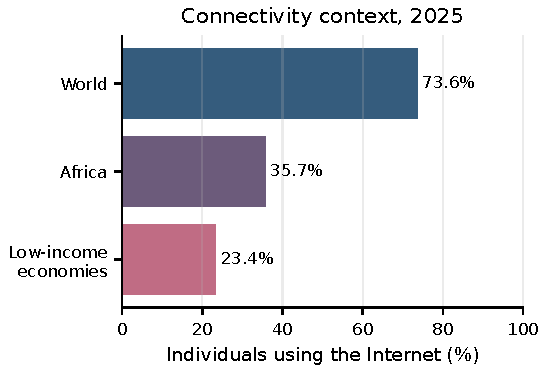
\includegraphics[width=\columnwidth]{figures/connectivity_context.pdf}
  \caption{Connectivity constraints relevant to digital-education architecture. Values are 2025 ITU estimates; the chart is generated from the included source-data file.}
  \label{fig:connectivity}
\end{figure}

\begin{figure}[t]
  \centering
  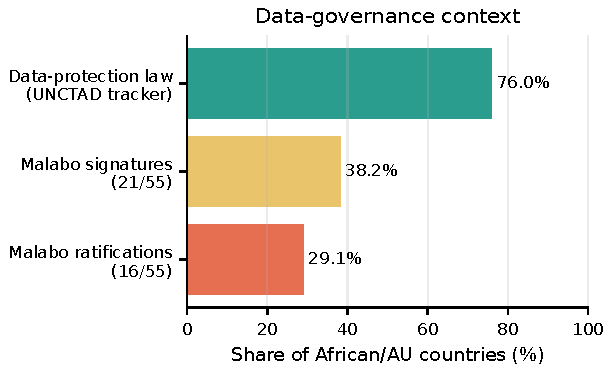
\includegraphics[width=\columnwidth]{figures/governance_context.pdf}
  \caption{Selected African data-governance indicators. The UNCTAD legislation indicator and AU treaty-status indicators use different concepts and denominators and are shown only as contextual signals.}
  \label{fig:governance}
\end{figure}


\begin{table*}[t]
\caption{Context Indicators Used to Motivate the Architecture (Not Evaluation Outcomes)}
\label{tab:context}
\centering
\footnotesize
\begin{tabularx}{\textwidth}{|p{0.18\textwidth}|p{0.11\textwidth}|p{0.15\textwidth}|Y|}
\hline
\THead{Indicator} & \THead{Value} & \THead{Source / date} & \THead{Architectural interpretation and caution} \\
\hline
Individuals using the Internet -- world & 73.6\% & ITU DataHub, 2025 \cite{itu2025} & Global benchmark used only to contextualize network-dependent service design. \\
\hline
Individuals using the Internet -- Africa & 35.7\% & ITU DataHub, 2025 \cite{itu2025} & Supports low-bandwidth, asynchronous, and bounded-offline requirements; it does not describe every country or institution. \\
\hline
Individuals using the Internet -- low-income economies & 23.4\% & ITU DataHub, 2025 \cite{itu2025} & Reinforces graceful degradation and non-smartphone alternatives. \\
\hline
African economies with data-protection/privacy legislation & 76.0\% & UNCTAD tracker, accessed 2026 \cite{unctadtracker} & Indicates broad legislative adoption, not harmonized rules, equivalent enforcement, or automatic transfer permission. \\
\hline
Malabo Convention signatures & 21/55 (38.2\%) & AU status list dated 8 July 2024 \cite{malabostatus} & Treaty participation is one governance signal among several; the denominator and date must remain explicit. \\
\hline
Malabo Convention ratifications/accessions & 16/55 (29.1\%) & AU status list dated 8 July 2024 \cite{malabostatus} & The architecture therefore uses reviewed jurisdiction profiles rather than a single assumed continental rule. \\
\hline
\end{tabularx}
\end{table*}

Security architecture must therefore address more than the classic perimeter. NIST defines zero trust as removing implicit trust based solely on network location or ownership and requiring explicit authentication and authorization for access to resources \cite{nist800207}. NIST SP 800-207A extends this logic to cloud-native and multi-location systems through application and service identities, gateways, and granular policies \cite{nist800207a}. However, zero trust does not by itself answer privacy questions such as whether a transfer is necessary, which fields are proportionate to a declared educational purpose, how learner rights are implemented, or how analytics should limit re-identification and inference. Privacy engineering and educational ethics must therefore be co-designed with access control \cite{nistprivacy,nist8062,hoelchen2018,jones2019}.

Existing research provides important partial solutions. Learning-analytics work analyzes consent, transparency, autonomy, and institutional maturity \cite{ifenthaler2016,hoelgriffiths2017,hoelchen2019,simic2025}. Research on micro-credentials emphasizes portability and stakeholder coordination \cite{ahsan2023,varadarajan2023}. Academic credential systems increasingly use cryptographic verification or distributed ledgers \cite{rustemi2024,wang2025}, while W3C Verifiable Credentials (VC) 2.0 now supplies a standards-based, machine-verifiable data model \cite{w3cvc20}. Yet the literature rarely joins these elements into an Africa-centered, jurisdiction-aware architecture that also treats low connectivity, workload identity, revocation, policy evidence, and privacy-preserving analytics as first-class concerns.

This paper addresses four research questions:
\begin{itemize}
  \item \textbf{RQ1:} Which security, privacy, governance, interoperability, and resilience requirements arise when African digital-education services exchange data and credentials across institutional and national boundaries?
  \item \textbf{RQ2:} How can zero-trust controls and privacy-enhancing mechanisms be combined without assuming a single continental legal regime, universal connectivity, or a shared raw-record repository?
  \item \textbf{RQ3:} Under an explicit synthetic workload, how do purpose, lawful-basis, jurisdiction, and minimization predicates affect false permits, prohibited-transfer blocking, legitimate denial, and data disclosure?
  \item \textbf{RQ4:} What analytical coverage, local computational cost, policy-staleness sensitivity, and differential-privacy utility are observed under reproducible protocols?
\end{itemize}

The contributions are fivefold. First, the paper derives fourteen traceable engineering requirements from continental instruments, representative national transfer rules, current standards, and peer-reviewed educational-privacy research. Second, it proposes a layered architecture joining subject, device, and workload identity with purpose- and jurisdiction-aware authorization. Third, it formalizes permit decisions as policy predicates that return obligations, including field projection, retention, encryption, evidence, and revocation hooks. Fourth, it evaluates the design through a declared threat-control rubric, a 3,000,000-request synthetic policy experiment, a differential-privacy utility study, a registry-staleness sensitivity analysis, and a local microbenchmark. Fifth, it supplies scripts, source data, raw measurements, and vector figures in an Overleaf-ready artifact. No learner records, biometric samples, production logs, or named-country performance data are used.

\section{Background and Related Work}
\subsection{Continental and National Governance Context}
The AU Data Policy Framework frames data as a strategic resource while emphasizing rights, security, interoperability, institutional coordination, and a shared African data space \cite{audatapolicy}. The 2025 AU Guidelines for Integrating Data Provisions in Protocols on Digital Trade reinforce harmonization and secure, inclusive cross-border data use \cite{audigitaltradeguidelines}. For digital education, these directions imply that portability cannot be reduced to moving complete learner databases between cloud regions. A safer interpretation is to make transfer decisions explicit, purpose-bound, evidence-producing, and limited to the minimum data needed for a particular interaction.

National rules remain decisive. Morocco's Law No. 09-08 establishes personal-data protections, and the Commission Nationale de Contr\^{o}le de la Protection des Donn\'{e}es \`{a} Caract\`{e}re Personnel (CNDP) provides a notification and authorization pathway for transfers abroad \cite{moroccolaw0908,cndptransfer}. Kenya's Data Protection Act addresses transfers outside Kenya in Sections 48--50, with further operational detail in the 2021 General Regulations \cite{kenyadpa,kenyaregulations}. South Africa's Protection of Personal Information Act (POPIA) includes transborder-flow conditions in Section 72 \cite{popia}. Institutions serving persons in the European Union may additionally confront the privacy-by-design and international-transfer requirements of GDPR Articles 25 and 44 \cite{gdpr}. These examples are not presented as an exhaustive legal survey. They demonstrate why an architecture should represent origin, destination, data category, purpose, legal basis, safeguards, retention, and downstream obligations as machine-enforceable attributes rather than static documentation.

The architecture in this paper is consequently \emph{law-aware but not law-determining}. It provides technical hooks and evidence for competent institutional and legal decision-makers; it does not declare a transfer lawful, replace regulator guidance, or infer that identical controls satisfy every jurisdiction.

\subsection{Zero Trust, Privacy Engineering, and Threat Modeling}
Zero trust shifts protection from network segments to resources and requires continuous evaluation of subjects, devices, services, and contextual risk \cite{nist800207}. Cloud-native implementation further requires application identities, ingress and egress gateways, service-mesh enforcement, and policies that travel across locations \cite{nist800207a}. This is especially relevant to education because an LMS, student-information system (SIS), assessment service, credential issuer, analytics pipeline, and payment service may be independently operated.

Privacy engineering adds objectives that conventional authorization does not express. The NIST Privacy Framework organizes privacy risk around identifying, governing, controlling, communicating, and protecting data processing \cite{nistprivacy}. NISTIR 8062 treats privacy as an engineering risk-management problem and encourages explicit privacy requirements and system-level analysis \cite{nist8062}. LINDDUN supplies a systematic vocabulary for privacy threats, including linkability, identifiability, non-repudiation, detectability, disclosure, unawareness, and non-compliance \cite{deng2011}. STRIDE-oriented security analysis, as operationalized in threat-modeling practice, complements it with spoofing, tampering, repudiation, information disclosure, denial of service, and elevation of privilege \cite{shostack2014}. The present threat model uses these frameworks as elicitation aids rather than claiming a formal certification against either method.

\subsection{Learning Analytics and Learner Autonomy}
Learning analytics can improve feedback and institutional decision-making, but centralizing fine-grained behavioral traces also creates surveillance, inference, and secondary-use risks. Hoel and Chen argue that educational benefit should constrain analytics design rather than allowing technical capability to define acceptable processing \cite{hoelchen2018}. Jones proposes informed-consent mechanisms that strengthen student privacy and autonomy \cite{jones2019}, while empirical work shows that students distinguish among data types and care about transparency and control \cite{ifenthaler2016}. Privacy frameworks influence system architecture, not merely notices and policies \cite{hoelgriffiths2017,hoelchen2019}. The HELA-CMM maturity model further suggests that sustainable analytics adoption requires organizational capabilities in addition to software features \cite{simic2025}. Accordingly, the architecture separates operational records from privacy-enhanced analytics and requires purpose, minimization, and privacy-budget obligations for higher-risk queries.

\subsection{Portable Credentials and Interoperability}
Micro-credentials promise flexible recognition, yet systematic reviews identify unresolved issues around quality assurance, comparability, institutional acceptance, and technical interoperability \cite{ahsan2023,varadarajan2023}. Blockchain-based diploma and identity models demonstrate the value of tamper evidence and decentralized verification \cite{rustemi2024,wang2025}; more recent work also combines zero-trust and decentralized-identity ideas for attack resistance \cite{emati2026}. Nevertheless, publishing raw personal or educational data to an immutable public ledger would conflict with minimization, correction, and erasure requirements. This paper therefore uses W3C VC 2.0 as the credential envelope, a trust registry for issuer metadata, and a privacy-preserving status mechanism for suspension or revocation \cite{w3cvc20,w3cstatus}. A ledger may anchor keys or governance records, but it is not required and must not hold raw learner data.

\begin{table*}[t]
\caption{Positioning Against Representative Standards and Research Streams}
\label{tab:related}
\centering
\scriptsize
\begin{tabularx}{\textwidth}{|p{0.15\textwidth}|p{0.19\textwidth}|p{0.27\textwidth}|p{0.31\textwidth}|}
\hline
\THead{Stream} & \THead{Representative evidence} & \THead{Primary contribution} & \THead{Gap addressed by \system} \\
\hline
Zero-trust architecture & NIST SP 800-207, SP 800-207A, SP 1800-35 \cite{nist800207,nist800207a,NIST180035_2025} & Resource-centric access, explicit verification, deployment patterns, workload and service controls. & Adds purpose limitation, jurisdiction-aware transfer predicates, field-level minimization, educational credential lifecycles, and low-connectivity behavior. \\
\hline
Digital identity and phishing resistance & NIST SP 800-63-4 and WebAuthn Level 3 \cite{Temoshok2025Identity,W3CWebAuthn2026} & Identity proofing, authentication assurance, federation, and public-key credentials. & Connects identity assurance to educational purpose, data category, destination profile, and decision obligations rather than treating authentication as sufficient authorization. \\
\hline
Attribute-based authorization & NIST SP 800-162 and service-mesh ABAC \cite{Hu2019ABAC,nist800204b} & Policy decisions over subject, object, operation, environment, and service attributes. & Adds legal/governance attributes, transfer admissibility, minimum claim views, evidence receipts, and freshness-aware policy registries. \\
\hline
Privacy engineering and learning analytics & NIST Privacy Framework; educational privacy and autonomy literature \cite{nistprivacy,nist8062,hoelchen2018,jones2019,simic2025} & Privacy-risk management, consent, transparency, autonomy, and institutional maturity. & Makes privacy obligations executable at access and transfer time and separates operational records from privacy-enhanced analytics. \\
\hline
Portable academic credentials & W3C VC 2.0, status list, micro-credential and diploma systems \cite{w3cvc20,w3cstatus,ahsan2023,rustemi2024,wang2025} & Tamper-evident claims, issuer-holder-verifier exchange, status, and credential portability. & Integrates credential verification with issuer governance, purpose-specific disclosure, revocation freshness, offline limits, and access policy. \\
\hline
Federated and privacy-preserving analytics & Federated learning, secure aggregation, differential privacy \cite{McMahan2017FL,Bonawitz2017SecureAgg,Dwork2006DP,gabrielli2022} & Distributed computation and bounded aggregate disclosure. & Places PET selection inside an educational governance workflow with cohort floors, budgets, query evidence, and residual-risk treatment. \\
\hline
African data and digital-education governance & AU Data Policy Framework, AU Digital Education Strategy, AfCFTA Digital Trade Protocol and guidelines \cite{audatapolicy,audigitaleducation,AfCFTADigitalTrade2024,audigitaltradeguidelines} & Harmonization, trusted data use, interoperability, digital transformation, and secure cross-border activity. & Translates policy directions into a common machine-enforceable schema while preserving institution- and jurisdiction-specific review. \\
\hline
\end{tabularx}
\end{table*}

\section{Research Design}
\subsection{Design-Science Process and Evidence Protocol}
The work follows the design-science sequence of problem identification, objective definition, artifact design, demonstration, evaluation, and communication \cite{peffers2007}. The evidence synthesis is structured and purposive rather than a claim of exhaustive systematic review. Official sources were prioritized for standards, treaty status, policy, and legislation; peer-reviewed sources were used for privacy, analytics, credentials, and design methodology. The evidence cutoff is \papercutoff.

The inclusion criteria were: (i) final standards or official instruments directly relevant to identity, privacy, cross-border transfer, digital education, or credentials; (ii) representative national rules from geographically and legally distinct African jurisdictions; (iii) peer-reviewed research with an explicit design, privacy, credential, or learning-analytics contribution; and (iv) sufficient bibliographic provenance for independent retrieval. Vendor marketing, undocumented product claims, unofficial legal summaries where primary text was available, and draft standards superseded by final recommendations were excluded. Table~\ref{tab:method} records the transformation from evidence to evaluation.

\begin{table}[t]
\caption{Design-Science and Evaluation Procedure}
\label{tab:method}
\centering
\scriptsize
\begin{tabularx}{\columnwidth}{|p{0.055\columnwidth}|p{0.27\columnwidth}|Y|}
\hline
\THead{Step} & \THead{Activity} & \THead{Traceable output} \\
\hline
1 & Problem framing & Assets, actors, trust boundaries, jurisdiction and connectivity constraints. \\
\hline
2 & Evidence synthesis & Primary standards and instruments plus peer-reviewed privacy, credential, and education research. \\
\hline
3 & Requirement derivation & Fourteen requirements with operational acceptance criteria. \\
\hline
4 & Artifact construction & Layered architecture, decision model, transfer workflow, credential lifecycle, and failure policy. \\
\hline
5 & Threat analysis & 12 threats $\times$ 3 objectives with declared 0/0.5/1 rubric and row-level rationales. \\
\hline
6 & Policy simulation & 3,000,000 synthetic requests, 30 seeds, two baselines, 95\% intervals, minimization and transfer metrics. \\
\hline
7 & Technical demonstration & DP utility, policy-staleness sensitivity, and single-host cryptographic/policy microbenchmark. \\
\hline
8 & Validity controls & Source primacy, declared assumptions, no real personal data, raw outputs, scripts, and environment metadata. \\
\hline
\end{tabularx}
\end{table}

\subsection{System Scope and Assumptions}
The target is a federation of higher-education, professional-training, and continuing-education platforms. In-scope assets are identity attributes, contact details, enrollment, grades, assessment submissions, credential claims, payment references, proctoring records, consent and rights requests, and learning-event data. In-scope actors are learners, educators, registrars, institutional administrators, employers, partner institutions, cloud or software providers, regulators, attackers, and malicious or coerced insiders.

The architecture assumes that each participating institution remains accountable for its own legal and educational decisions; cryptographic keys are managed through institutionally controlled key-management or hardware-security boundaries; jurisdiction profiles are reviewed by competent personnel; and service identities can be provisioned. It does \emph{not} assume uniform law, constant connectivity, universal smartphone ownership, a public blockchain, or mutual trust among every participant.

\subsection{Derived Requirements}
Table~\ref{tab:reqs} presents the requirements. Their purpose is not to encode legislation directly, but to translate recurring obligations and risks into testable system behavior.

\begin{table*}[t]
\caption{Traceable Engineering Requirements and Acceptance Evidence}
\label{tab:reqs}
\centering
\scriptsize
\begin{tabularx}{\textwidth}{|p{0.035\textwidth}|p{0.135\textwidth}|p{0.37\textwidth}|Y|}
\hline
\THead{ID} & \THead{Requirement} & \THead{Operational interpretation} & \THead{Minimum acceptance evidence} \\
\hline
R1 & Explicit identities & Authenticate the human subject, device context, and calling workload before protected-resource access. & Distinct subject/device/workload assertions; issuer and audience verification; expired or wrong-audience assertions denied. \\
\hline
R2 & Phishing-resistant access & Prefer public-key authenticators for privileged and high-impact workflows; bind recovery to risk and audit. & Passkey/WebAuthn test for privileged roles; recovery simulation; step-up and revocation logs \cite{Temoshok2025Identity,W3CWebAuthn2026}. \\
\hline
R3 & Least privilege & Issue short-lived, resource- and action-scoped authorization and re-evaluate high-risk actions. & Deny-path tests for role, relationship, action, expiry, and device-risk changes \cite{nist800207,nist800207a}. \\
\hline
R4 & Purpose limitation & Require a declared, allowed educational purpose independent of the user's broad role. & Purpose catalog; policy tests showing identical role/resource pairs produce different decisions by purpose. \\
\hline
R5 & Governed transfer & Evaluate origin, destination, category, purpose, basis/safeguard, recipient assurance, retention, and onward transfer. & Versioned jurisdiction profiles; blocked-transfer tests; approval evidence and decision receipt \cite{audigitaltradeguidelines,cndptransfer,kenyadpa,popia}. \\
\hline
R6 & Data minimization & Release only the fields/claims required by the approved purpose and destination profile. & Field-projection tests; schema diff; denied access to non-projected fields; minimization metrics. \\
\hline
R7 & Regional authority & Keep authoritative records in approved zones and exchange bounded claim views instead of default database replication. & Data-flow map; key-domain separation; recipient cannot dereference a minimized view into the source record. \\
\hline
R8 & Learner rights & Support notice/consent where applicable, correction, export, objection, deletion/retention decisions, and appeal. & Rights-request workflow, identity verification, decision rationale, completion timestamps, and audit trail \cite{nistprivacy,jones2019}. \\
\hline
R9 & Credential integrity & Verify issuer trust, signature, schema, validity period, audience, and status; separate cryptographic validity from academic recognition. & Positive/negative VC vectors, revoked/suspended status tests, unknown-issuer denial, and issuer-governance record \cite{w3cvc20,w3cstatus}. \\
\hline
R10 & Privacy-enhanced analytics & Prefer aggregation/federation where raw-event pooling is unnecessary; apply cohort floors, clipping, budgets, and query evidence. & Privacy-budget ledger, repeated-query tests, small-cohort denial, model leakage assessment \cite{Dwork2006DP,McMahan2017FL,Bonawitz2017SecureAgg}. \\
\hline
R11 & Continuous telemetry & Correlate identity, device, workload, gateway, egress, data-access, and credential-status events. & Common event schema, time synchronization, anomaly detection, alert-to-containment drill, and retention policy. \\
\hline
R12 & Low-connectivity resilience & Support local-first content, compact tokens, asynchronous audit buffering, and bounded offline verification. & Packet-loss/offline tests; freshness-window enforcement; queued-event reconciliation; fail-closed tests for high-risk operations. \\
\hline
R13 & Coordinated response & Support session and credential revocation, key rotation, transfer suspension, evidence preservation, and notification workflow. & Incident playbook, key-rotation drill, status propagation test, transfer scoping, and restoration evidence. \\
\hline
R14 & Accountability and portability & Sign decision receipts, version policies, test configurations, retain open exports, and exercise vendor exit. & Receipt verification, policy rollback test, configuration diff, standards-based export, and documented migration rehearsal. \\
\hline
\end{tabularx}
\end{table*}

\section{Proposed Reference Architecture}
\subsection{Design Principles}
The architecture is guided by six principles. First, \emph{verify each access path}: subject, device, and workload identities are distinct signals. Second, \emph{make purpose enforceable}: an authorization request without an approved educational purpose cannot be permitted merely because the user has a broad role. Third, \emph{move claims rather than databases}: authoritative records remain in controlled zones, while cross-border services receive purpose-specific views. Fourth, \emph{separate evidence from exposure}: immutable or append-only records contain decision metadata and digests, not raw personal data. Fifth, \emph{degrade safely}: offline or low-bandwidth behavior is bounded by risk and freshness. Sixth, \emph{prefer interoperable interfaces}: identity, credentials, status, policy schemas, and exports should not require a single vendor.

\begin{figure*}[t]
  \centering
  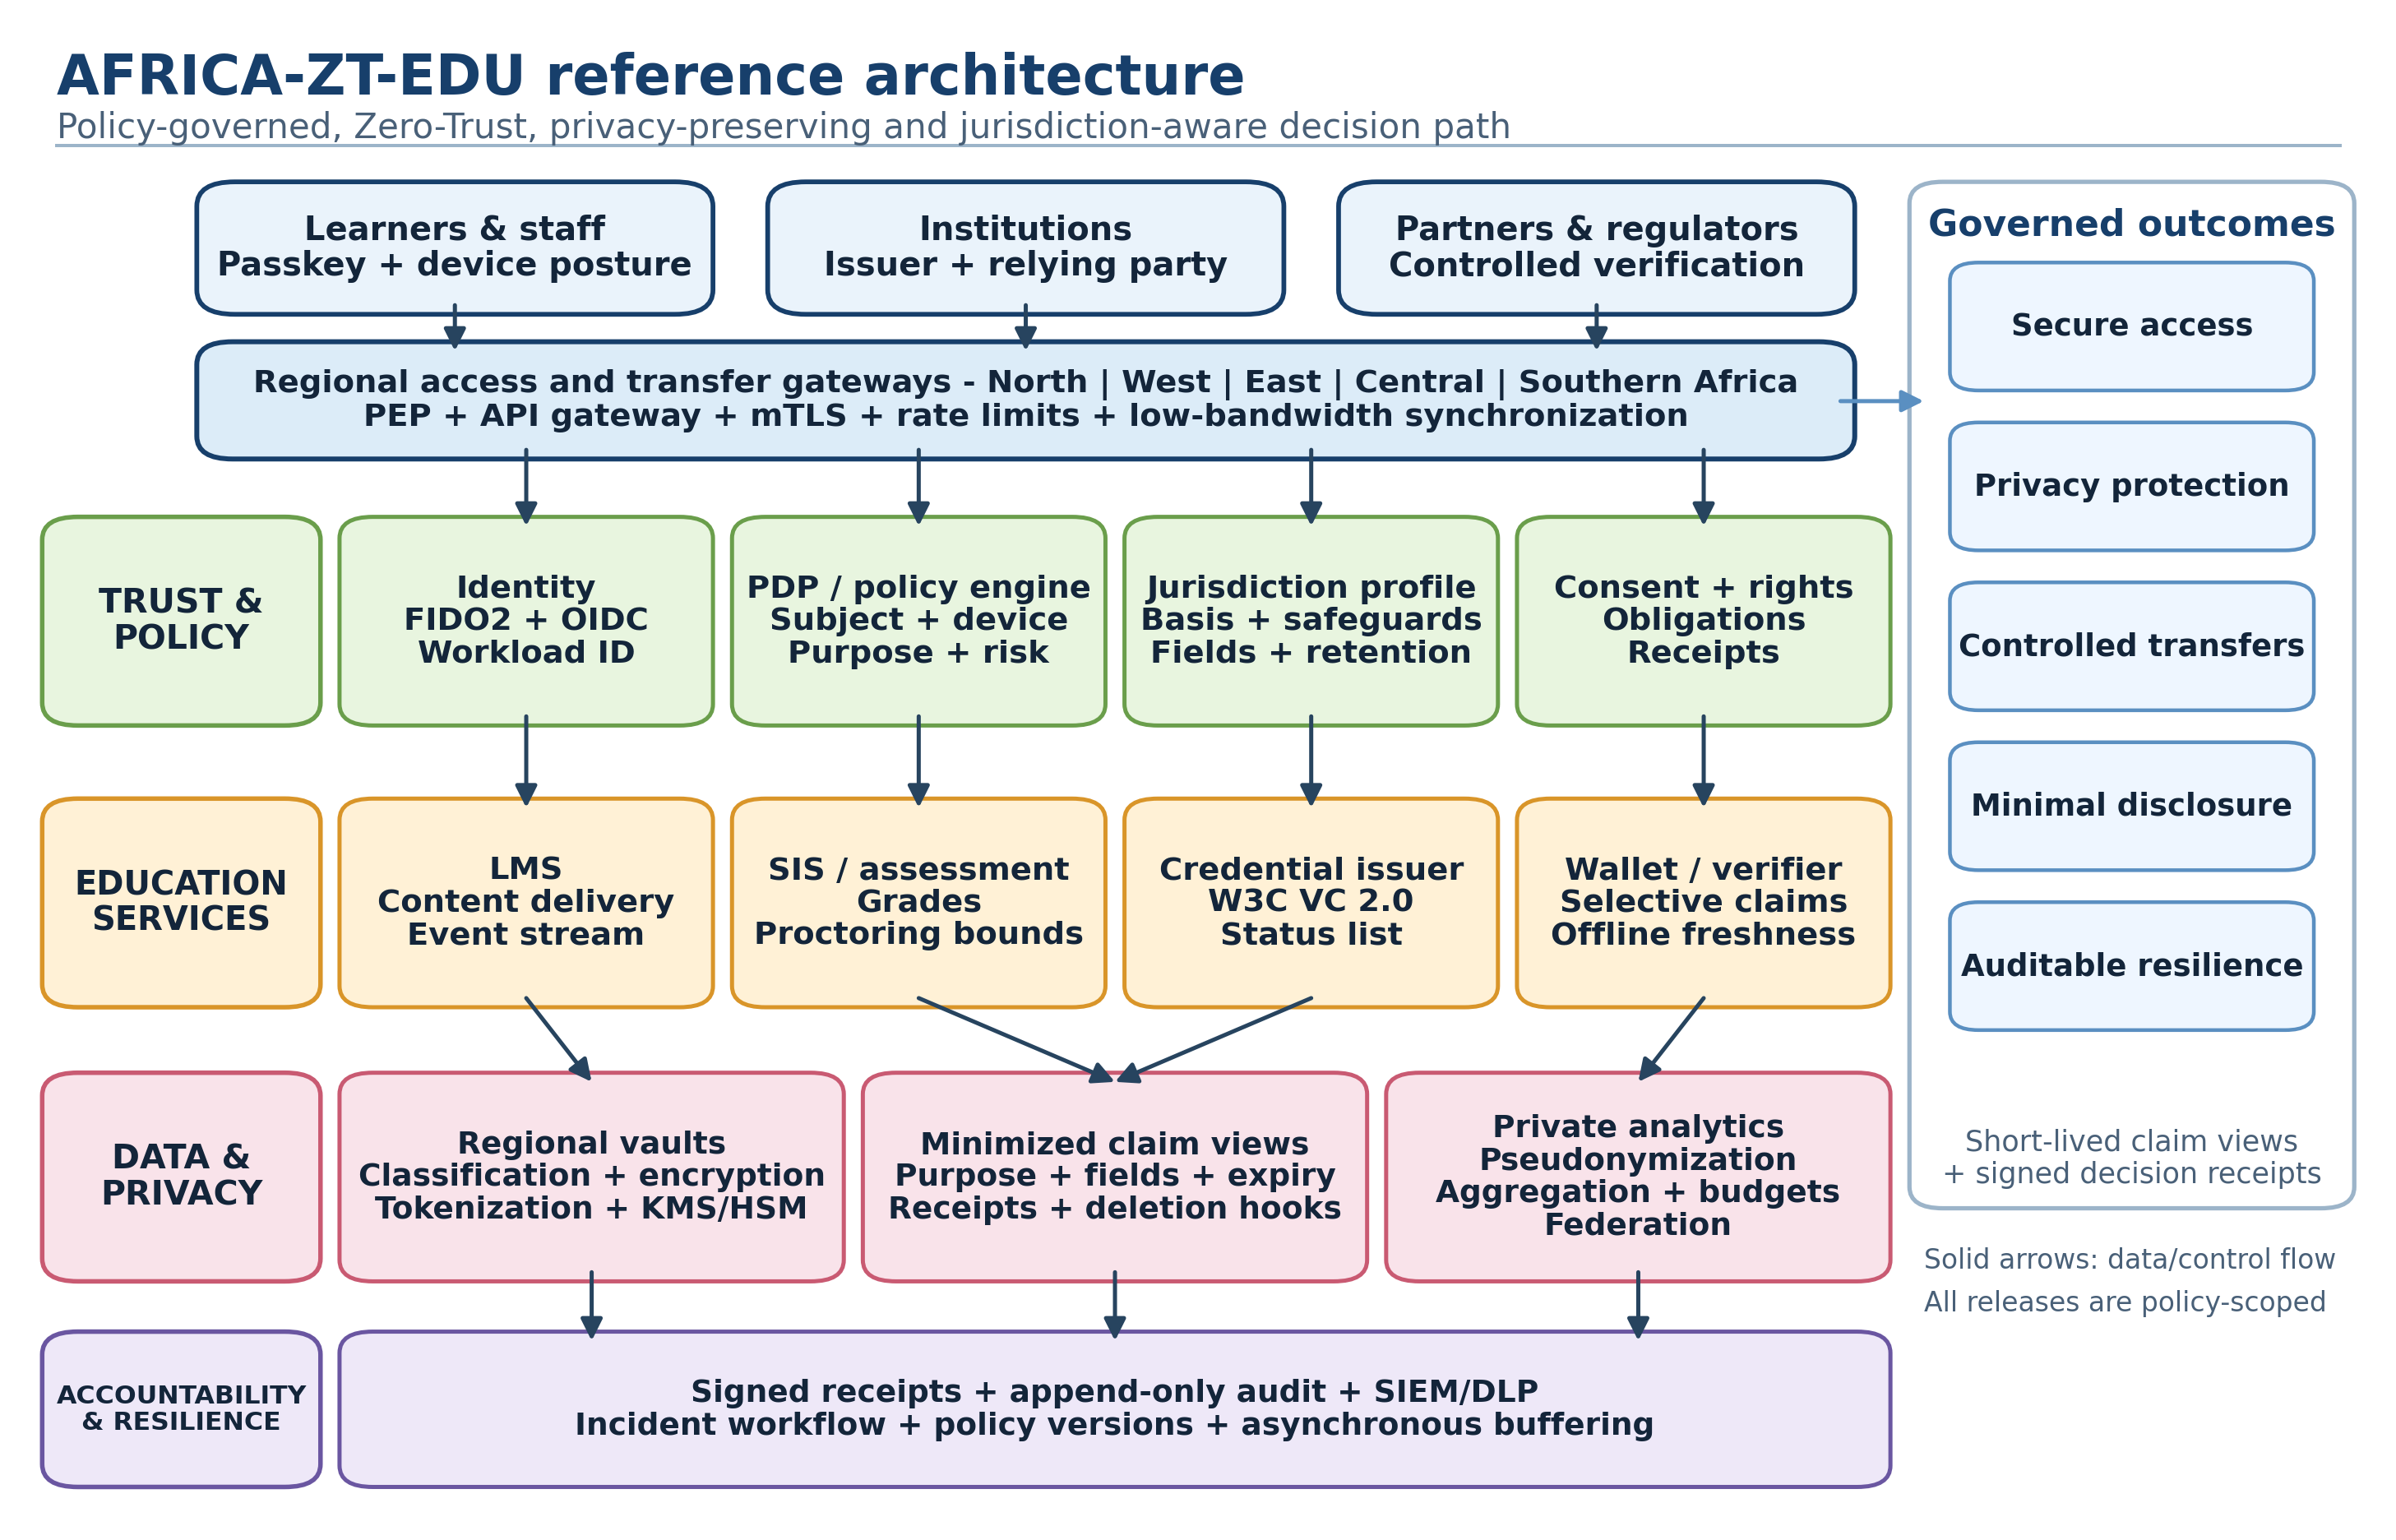
\includegraphics[width=\textwidth]{figures/reference_architecture_v3.png}
  \caption{Proposed reference architecture. A policy decision joins identity, device, workload, purpose, risk, jurisdiction, transfer basis, and minimization obligations before regional data zones release a claim view. The high-resolution diagram is an implementation-neutral logical model; arrows are routed outside component boxes to preserve traceability and legibility.}
  \label{fig:architecture}
\end{figure*}

\subsection{Decision Model}
An access or transfer request is represented as
\begin{equation}
q=\langle s,d,w,r,a,p,j_o,j_d,c,b,t\rangle,
\end{equation}
where $s$ is the subject, $d$ the device context, $w$ the workload identity, $r$ the resource, $a$ the action, $p$ the declared purpose, $j_o$ and $j_d$ the origin and destination jurisdictions, $c$ the data category, $b$ the transfer basis or approved safeguard profile, and $t$ the temporal context.

A permit decision is issued only if
\begin{equation}
\begin{split}
\operatorname{Permit}(q) \Leftrightarrow {} & A_s(s) \land A_d(d) \land A_w(w) \\
& \land L(s,r,a,p) \land X(j_o,j_d,c,p,b) \\
& \land M(r,p,c) \land \rho(q) < \tau,
\end{split}
\label{eq:permit}
\end{equation}
where $A_s$, $A_d$, and $A_w$ are authentication predicates; $L$ is the local authorization predicate; $X$ is the jurisdiction and transfer predicate; $M$ verifies that the selected field set is no larger than the purpose-specific allow-list; $\rho(q)$ is a risk score; and $\tau$ is the applicable threshold. A positive decision returns obligations rather than a bare Boolean:
\begin{equation}
O(q)=\{F,\;T_{\mathrm{exp}},\;E,\;R_t,\;\Gamma,\;\Delta\},
\end{equation}
where $F$ is the field projection, $T_{\mathrm{exp}}$ the token or view expiry, $E$ encryption requirements, $R_t$ retention, $\Gamma$ logging and notification duties, and $\Delta$ downstream deletion or revocation hooks. This structure allows an institution to change a jurisdiction profile without rewriting every application.

\begin{table*}[t]
\caption{Authorization Input Attributes and Example Evidence}
\label{tab:attributes}
\centering
\scriptsize
\begin{tabularx}{\textwidth}{|p{0.12\textwidth}|p{0.31\textwidth}|p{0.25\textwidth}|Y|}
\hline
\THead{Category} & \THead{Core attributes} & \THead{Illustrative evidence source} & \THead{Security/privacy purpose} \\
\hline
Subject & Stable or pairwise identifier, role, affiliation, assurance level, relationship, delegation. & Institutional IdP, verified credential, registrar relationship service. & Establish who is requesting and the relationship to the resource without relying on network location. \\
\hline
Device/session & Device posture, authenticator type, session age, token binding, anomaly/risk signals. & Device trust service, WebAuthn assertion, session telemetry. & Reduce account-takeover and replay risk; trigger step-up or denial. \\
\hline
Workload & Service identifier, deployment identity, software provenance, calling chain, certificate/key state. & Workload identity system, mTLS certificate, signed deployment metadata. & Prevent one service from inheriting another service's privileges. \\
\hline
Resource/action & Resource class, owner/tenant, sensitivity, action, volume, field set, export flag. & Data catalog, API schema, object metadata, request. & Apply least privilege, rate/volume limits, and field projection. \\
\hline
Purpose/basis & Declared purpose, compatible use, legal/governance basis, approval state, retention reason. & Purpose catalog, consent/contract/mandate registry, review workflow. & Prevent secondary use and make purpose enforceable rather than documentary. \\
\hline
Jurisdiction/recipient & Origin, destination, recipient class, assurance, transfer condition, onward-transfer rule. & Reviewed jurisdiction profile, partner registry, contract/safeguard metadata. & Decide whether a cross-border release is permitted and under which obligations. \\
\hline
Time/status/risk & Policy version, time, credential/status freshness, threat signals, emergency state. & Policy registry, status list, SIEM, risk engine. & Bound offline use, prevent rollback, and adapt decisions to current risk. \\
\hline
\end{tabularx}
\end{table*}

\begin{table}[t]
\caption{Decision Outcomes and Mandatory Effects}
\label{tab:outcomes}
\centering
\scriptsize
\begin{tabularx}{\columnwidth}{|p{0.29\columnwidth}|Y|}
\hline
\THead{Outcome} & \THead{Mandatory effect} \\
\hline
Permit & Release the approved minimized view with short expiry and record policy/evidence metadata. \\
\hline
Permit with obligations & Enforce field projection, encryption, retention, notification, rate, deletion, and downstream-use constraints. \\
\hline
Step-up required & Obtain stronger subject/device assurance or dual approval, then re-evaluate the entire request. \\
\hline
Manual review & Pause release; route to a competent institutional role with the evaluated facts and policy version. \\
\hline
Deny & Release no protected values; return a non-sensitive reason category and preserve audit evidence. \\
\hline
Emergency permit & Use only an authorized break-glass policy; minimize fields, shorten expiry, alert reviewers, and require post-event review. \\
\hline
\end{tabularx}
\end{table}


\subsection{Identity, Device, and Workload Plane}
Learners and staff authenticate through federated OpenID Connect or equivalent institutional identity, with phishing-resistant passkeys preferred for higher-risk roles. Device posture is a contextual signal, not a permanent identity guarantee. Services receive distinct workload identities, preferably short-lived and automatically rotated, so that an LMS calling a credential issuer is not authorized merely because both applications reside in the same virtual network. Policy-enforcement points (PEPs) at APIs and service gateways send normalized requests to a policy decision point (PDP), which evaluates Equation~\eqref{eq:permit}. High-risk actions---such as bulk grade export, proctoring-data access, key administration, or cross-border release of special-category data---require stronger device posture, step-up authentication, or dual approval.

\subsection{Jurisdiction-Aware Transfer Gateway}
The transfer gateway is the architectural distinction between ordinary attribute-based access control and governed cross-border processing. A jurisdiction registry contains reviewed policy profiles: recognized purposes, data categories, prohibited fields, approved bases or safeguards, retention ceilings, recipient classes, onward-transfer constraints, and incident contacts. A transfer request must identify the recipient and declared purpose; the PDP then selects a field projection and obligations. The gateway records a signed decision receipt containing policy version, request digest, decision, selected fields, expiry, destination, and responsible institutional role. Raw values are not written to the receipt.

Table~\ref{tab:legalmap} illustrates the mapping. The entries are engineering interpretations for traceability, not legal opinions.

\begin{table*}[t]
\caption{Illustrative Instrument-to-Architecture Mapping}
\label{tab:legalmap}
\centering
\scriptsize
\begin{tabularx}{\textwidth}{|p{0.19\textwidth}|p{0.34\textwidth}|Y|}
\hline
\THead{Instrument or source} & \THead{Engineering implication} & \THead{Architecture mechanism} \\
\hline
AU Data Policy Framework \cite{audatapolicy} & Harmonization, rights protection, trust, shared data spaces, and accountable use should coexist. & Common policy schema, regional data zones, rights workflow, portable receipts, and standards-based interfaces. \\
\hline
AU Digital Education Strategy \cite{audigitaleducation} & Adoption must account for skills, devices, networks, languages, and institutional capacity. & Low-bandwidth synchronization, local-first content, staged deployment, and bounded offline credential verification. \\
\hline
AfCFTA Digital Trade Protocol and AU data guidelines \cite{AfCFTADigitalTrade2024,audigitaltradeguidelines} & Cross-border digital activity should be trustworthy, interoperable, transparent, and supported by common principles. & Jurisdiction registry, transfer predicate, safeguard metadata, interoperable APIs, and evidence-producing gateways. \\
\hline
Malabo Convention \cite{malaboconvention} & Cybersecurity and personal-data protection require organizational and technical safeguards and coordinated accountability. & Security/privacy co-design, incident workflow, key rotation, transfer suspension, and evidence preservation. \\
\hline
Morocco Law 09-08 and CNDP process \cite{moroccolaw0908,cndptransfer} & International transfers may require a documented condition, procedure, or authorization. & Transfer-basis attribute, workflow state, destination profile, approval evidence, and receipt. \\
\hline
Kenya Data Protection Act and Regulations \cite{kenyadpa,kenyaregulations} & Transfer conditions and safeguards must be demonstrable. & Safeguard profile, recipient assurance, category rules, and auditable transfer register. \\
\hline
South Africa POPIA Sec. 72 \cite{popia} & Transborder processing depends on recipient protections or another recognized condition. & Destination assurance, contractual/safeguard metadata, purpose, necessity, and onward-transfer checks. \\
\hline
GDPR Arts. 25 and 44 \cite{gdpr} & Privacy by design/default and controlled international transfers affect institutions handling EU-linked data. & Default-minimized projections, transfer predicate, retention obligations, rights workflow, and accountability evidence. \\
\hline
W3C VC 2.0 and status list \cite{w3cvc20,w3cstatus} & Credentials should be interoperable, verifiable, privacy-respecting, and lifecycle-managed. & Issuer/verifier interfaces, selective presentation, trust registry, signed status, and freshness policy. \\
\hline
\end{tabularx}
\end{table*}

\subsection{Regional Data and Privacy Plane}
Authoritative SIS and assessment records are placed in approved encrypted data zones. Fields are classified by sensitivity and purpose, with independent keys or envelope-encryption domains for identity, academic, financial, and proctoring data. Tokenization or pseudonymization reduces exposure to analytics and support services. A cross-border recipient receives a time-bounded claim view, such as ``credential valid, six credits, distinction band,'' rather than the learner's full profile and event history.

For analytics, the platform prefers aggregate or federated computation when the educational question does not require raw-event pooling. Privacy budgets, minimum cohort sizes, query logging, and disclosure review can reduce inference risk. These mechanisms do not make analytics risk-free: trained models may retain information, small populations can be re-identified, and institutional incentives can expand purposes. The architecture therefore leaves residual risk for T9 rather than assigning full analytical coverage.

\subsection{Credential Lifecycle}
An institution issues a VC after its internal academic decision is complete. The credential contains only required claims, an issuer identifier, validity information, and a status reference. The holder stores it in a wallet or institution-provided account. A verifier requests a claim set tied to a declared purpose; the holder or presentation service discloses only those claims. The verifier validates issuer metadata, signature, schema, time bounds, and status freshness. High-risk decisions fail closed when current status cannot be obtained. Lower-risk verification may use a signed cached status object within a formally bounded offline window, with the stale-state condition recorded in the decision receipt.

This design deliberately separates academic truth from cryptographic proof. A signature proves origin and integrity, not educational quality or legal recognition. Governance bodies must still define issuer eligibility, assurance levels, appeals, corrections, and revocation authority. The credential layer therefore complements rather than replaces quality assurance.

\subsection{Low-Connectivity and Failure Modes}
Connectivity constraints in Fig.~\ref{fig:connectivity} affect every control. The design supports compact tokens, progressive synchronization, offline content packages, local queues for signed audit events, and asynchronous policy updates with version checks. Availability is risk-tiered: routine content access can continue from a local cache; credential presentation can continue within a signed freshness window; but bulk export, administrator elevation, key changes, and sensitive transfer are denied when central policy or current status is unavailable. When connectivity returns, queued audit events are hash-linked, time-checked, and reconciled. Conflict handling favors the most restrictive valid policy version unless an authorized emergency procedure is invoked and separately recorded.

\section{Threat Model and Evaluation}
\subsection{Threat Elicitation}
The threat model combines security and privacy prompts from STRIDE and LINDDUN \cite{shostack2014,deng2011}. Trust boundaries occur between user devices and access gateways, gateways and the PDP, services and regional data zones, credential issuers and wallets, institutions and external verifiers, and operational systems and analytics. Table~\ref{tab:threats} summarizes twelve high-priority threats. It is not an exhaustive attack tree; rather, it is the evaluation frame for the reference architecture.

\begin{table*}[t]
\caption{Threat Set, Principal Controls, and Residual Concerns}
\label{tab:threats}
\centering
\scriptsize
\begin{tabularx}{\textwidth}{|p{0.035\textwidth}|p{0.18\textwidth}|p{0.37\textwidth}|Y|}
\hline
\THead{ID} & \THead{Threat} & \THead{Principal architecture controls} & \THead{Important residual concern} \\
\hline
T1 & Phishing/account takeover & Passkeys, device context, risk-aware PDP, short-lived tokens, recovery controls, rapid revocation. & Recovery and social-engineering processes remain exploitable. \\
\hline
T2 & Stolen bearer/session token & Proof-bound or mutually authenticated tokens, context checks, replay analytics, resource scope \cite{rfc8705,rfc9449}. & A compromised client can act within a still-valid session. \\
\hline
T3 & Compromised endpoint & Device posture, step-up, per-resource decisions, least privilege, containment. & Posture signals are incomplete and may be forged or delayed. \\
\hline
T4 & Overprivileged administrator & Just-in-time privilege, purpose constraints, dual approval, segregated keys, decision receipts. & Authorized insiders can collude or misuse legitimate workflows. \\
\hline
T5 & Unlawful/excessive transfer & Jurisdiction registry, transfer predicate, field projection, expiry, recipient assurance, approval evidence. & Incorrect legal profiles or institutional interpretation can authorize an improper flow. \\
\hline
T6 & API scraping/exfiltration & Workload identity, rate/volume controls, egress DLP, field minimization, anomaly detection. & Slow distributed extraction may evade thresholds. \\
\hline
T7 & Credential forgery & Issuer signatures, trust registry, schema validation, status verification, verifier receipts. & Compromised issuer keys or fraudulent issuers remain governance risks. \\
\hline
T8 & Revocation bypass & Signed status, freshness policy, high-risk fail-closed behavior, bounded cached status. & Offline acceptance creates a deliberate time-limited exposure window. \\
\hline
T9 & Analytics inference/privacy leakage & Pseudonymization, aggregation, cohort floors, privacy budgets, secure aggregation, federated analysis. & Models, repeated queries, and small populations can retain or reveal information. \\
\hline
T10 & Audit tampering/repudiation & Signed receipts, append-only storage, hash linkage, key segregation, replication. & Endpoint compromise can falsify events before capture. \\
\hline
T11 & Disruption/intermittent connectivity & Regional zones, local-first content, bounded offline verification, asynchronous buffering. & Severe outages and device loss still interrupt high-risk operations. \\
\hline
T12 & Lock-in/policy misconfiguration & Open standards, policy as code, conformance tests, simulation, versioned rollback, portable exports. & Semantic errors and proprietary extensions cannot be eliminated architecturally. \\
\hline
\end{tabularx}
\end{table*}

\subsection{Analytical Coverage Rubric}
Each threat is scored across three objectives: (i) prevent or minimize; (ii) detect or verify; and (iii) contain, recover, or account. A score of 0 means the reference profile contains no explicit mechanism; 0.5 means a partial, manually dependent, or non-integrated mechanism; and 1 means the architecture contains an explicit, traceable mechanism. The perimeter-centric reference profile assumes password-centered authentication, optional MFA, static broad roles, ordinary centralized logs, generic encryption in transit and at rest, application-specific revocation, cloud redundancy, and manual cross-border review. It is a constructed comparator, not a measurement of a named product.

The proposed architecture scores 34 of 36 possible points (94.4\%), while the comparator scores 15 of 36 (41.7\%). Figure~\ref{fig:coverage} shows per-threat results. Full scores are withheld for analytics leakage because privacy loss cannot always be detected or reversed; for connectivity disruption because monitoring itself can fail; and for policy misconfiguration because conformance tests do not prove semantic correctness. The scoring demonstrates requirement-to-control traceability, not exploit resistance. Independent red-team testing and operational evidence are required before deployment claims.

\begin{figure*}[t]
  \centering
  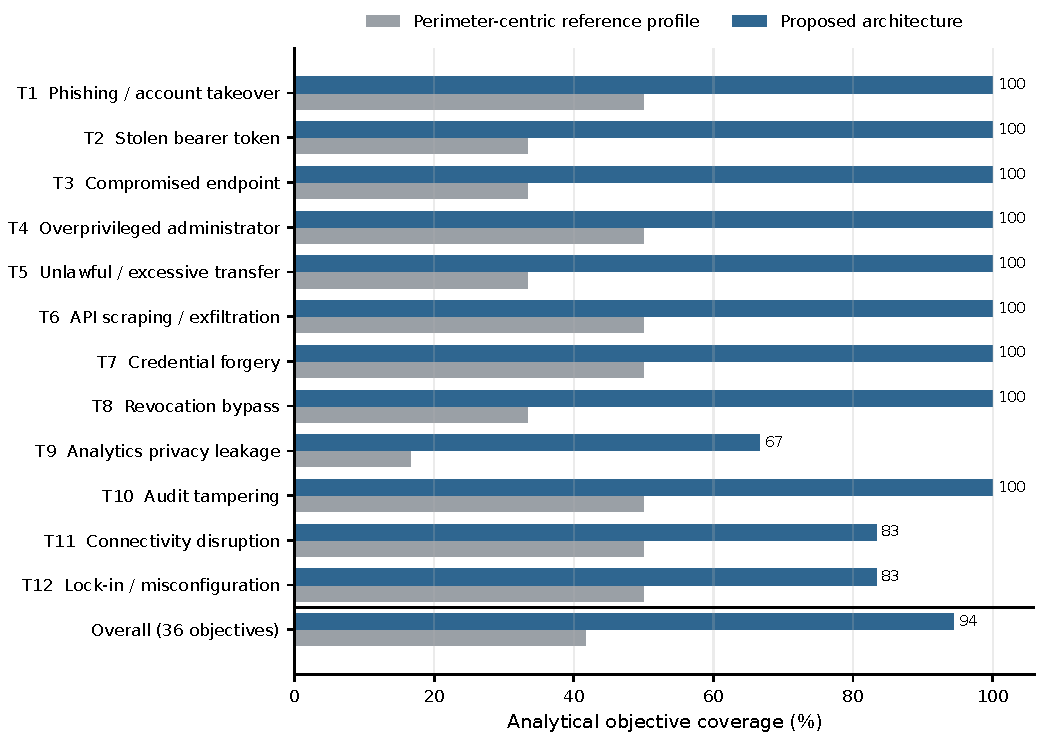
\includegraphics[width=0.95\textwidth]{figures/threat_coverage.pdf}
  \caption{Analytical coverage under the declared 0/0.5/1 rubric. The proposed design reaches 34/36 objectives; the constructed perimeter-centric reference profile reaches 15/36. Values represent explicit architectural control presence, not empirical breach probability.}
  \label{fig:coverage}
\end{figure*}


\subsection{Synthetic Policy-Expressiveness Evaluation}
The second evaluation component tests whether the proposed predicates express a declared synthetic policy truth more precisely than two baselines. It does not estimate real attack frequency, institutional error rates, or legal compliance. The generator creates 100,000 requests for each of 30 independent seeds, producing 3,000,000 decisions. Twenty-four synthetic institutions are distributed across 12 abstract jurisdiction profiles; no country names are assigned. Four profiles are configured in each of three experimental classes: strict residency, conditional transfer, and interoperable/trusted flow. These labels are test constructs rather than assessments of actual jurisdictions.

Requests contain six roles, six resource classes, five actions, six purposes, five basis states, identity assurance, device posture, session age, relationship state, risk, source and destination profiles, and cross-border status. Thirty-eight percent of requests are configured to cross a jurisdiction. A controlled 18\% misuse tail independently samples role/resource/action combinations. Resource schemas contain 8--24 fields, and purpose-specific release profiles contain 2--9 fields. Across seeds, 24.572\% of requests satisfy all ground-truth predicates; this is an intentionally stress-oriented distribution, not a traffic estimate.

\begin{table*}[t]
\caption{Synthetic Policy-Evaluation Configuration}
\label{tab:simconfig}
\centering
\footnotesize
\begin{tabularx}{\textwidth}{|p{0.20\textwidth}|p{0.25\textwidth}|Y|}
\hline
\THead{Parameter} & \THead{Configured value} & \THead{Interpretation / validity boundary} \\
\hline
Requests and repetitions & 100,000 per seed; 30 independent seeds; 3,000,000 total & Confidence intervals summarize between-seed variation under a fixed generator. \\
\hline
Institutions and jurisdictions & 24 synthetic institutions; 12 abstract profiles & No real institution or country is represented, ranked, or assigned a result. \\
\hline
Intended cross-border share & 38\% & Produces enough cross-jurisdiction cases for transfer-policy stress testing. \\
\hline
Policy classes & Strict residency, conditional transfer, interoperable/trusted flow & Abstract generator classes, not legal labels for countries. \\
\hline
Baselines & Legacy RBAC; contextual zero-trust ABAC & Legacy uses coarse role/resource/action logic; ABAC adds context but omits purpose, basis, and jurisdiction predicates. \\
\hline
Proposed design & Contextual ABAC + purpose + basis + jurisdiction + minimization + receipt & Tests the incremental expressiveness of the complete decision model. \\
\hline
Policy staleness in main run & 0.25\% false-allow and 0.10\% false-deny transfer entries & Models registry error explicitly; it is not inferred from observed institutions. \\
\hline
Modeled latency scope & In-process synthetic policy components; network RTT excluded & Used only for relative architectural modeling, not deployment capacity planning. \\
\hline
DP utility study & 50,000 synthetic cohort-count queries; $\epsilon\in\{0.25,0.5,1,2,4,8\}$ & Illustrates a privacy-utility trade-off; no learner outcome is analyzed. \\
\hline
\end{tabularx}
\end{table*}

Let $y_i\in\{0,1\}$ be the ground-truth permit label and $\hat y_i$ the architecture decision. The false-permit rate is calculated over invalid requests,
\begin{equation}
\operatorname{FPR}=\frac{\sum_i \mathbb{1}(\hat y_i=1\land y_i=0)}{\sum_i \mathbb{1}(y_i=0)},
\end{equation}
while permit precision is $\sum_i\mathbb{1}(\hat y_i=1\land y_i=1)/\sum_i\mathbb{1}(\hat y_i=1)$. The prohibited-transfer block rate is evaluated only over requests that pass contextual, purpose, and basis checks but fail the ground-truth cross-border predicate. The field metric is the mean number of released fields over permitted requests. For each metric, the artifact reports the mean across 30 seeds and a two-sided 95\% normal-approximation interval, $\bar{x}\pm1.96s/\sqrt{30}$. The raw per-seed values are included so alternative intervals can be computed.

\begin{table*}[t]
\caption{Policy-Evaluation Results Across 30 Seeds (Mean and 95\% Confidence Interval)}
\label{tab:policyresults}
\centering
\scriptsize
\begin{tabularx}{\textwidth}{|p{0.18\textwidth}|C|C|C|C|C|C|}
\hline
\THead{Architecture} & \THead{False permit \%} & \THead{Permit precision \%} & \THead{Legitimate denial \%} & \THead{Blocked prohibited transfer \%} & \THead{Mean fields disclosed} & \THead{Modeled p95 ms} \\
\hline
Legacy RBAC & 77.042 [76.978, 77.106] & 29.718 [29.663, 29.773] & 0.000 [0.000, 0.000] & 0.000 [0.000, 0.000] & 12.702 [12.691, 12.712] & 1.917 [1.915, 1.919] \\
\hline
Zero-Trust ABAC & 10.039 [9.995, 10.084] & 76.442 [76.353, 76.532] & 0.000 [0.000, 0.000] & 0.000 [0.000, 0.000] & 12.702 [12.691, 12.712] & 6.344 [6.338, 6.349] \\
\hline
\system & \textbf{0.0095 [0.0082, 0.0108]} & \textbf{99.971 [99.967, 99.975]} & 0.104 [0.095, 0.112] & \textbf{99.750 [99.716, 99.785]} & \textbf{4.920 [4.917, 4.924]} & 9.121 [9.114, 9.128] \\
\hline
\end{tabularx}
\end{table*}

\begin{figure*}[t]
\centering
\subfloat[False permits among policy-invalid requests.]{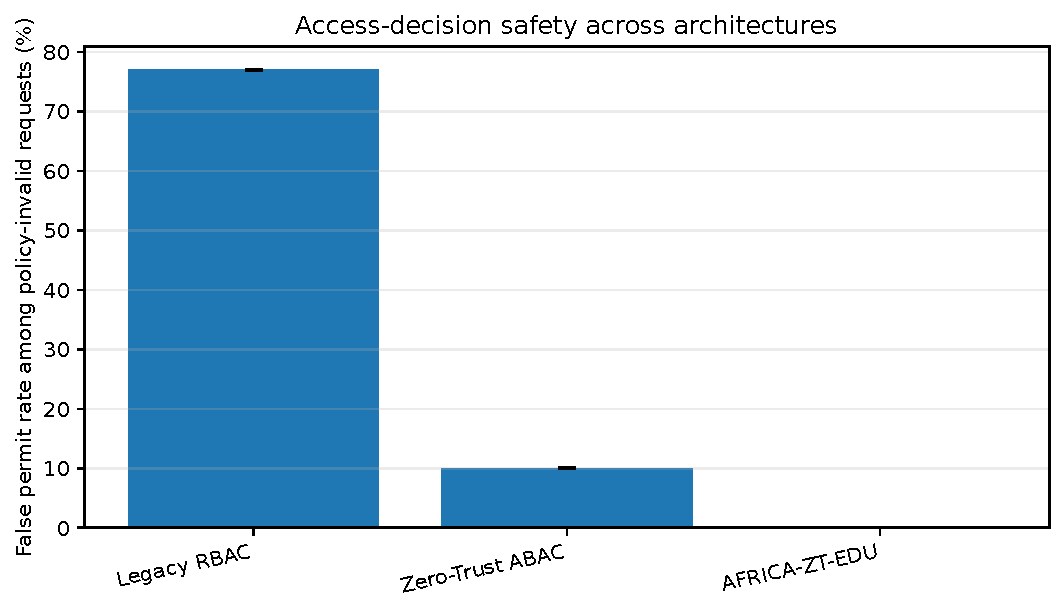
\includegraphics[width=0.49\textwidth]{figures/false_permit_rate.pdf}\label{fig:falsepermit}}
\hfill
\subfloat[Blocked otherwise-authorized prohibited transfers.]{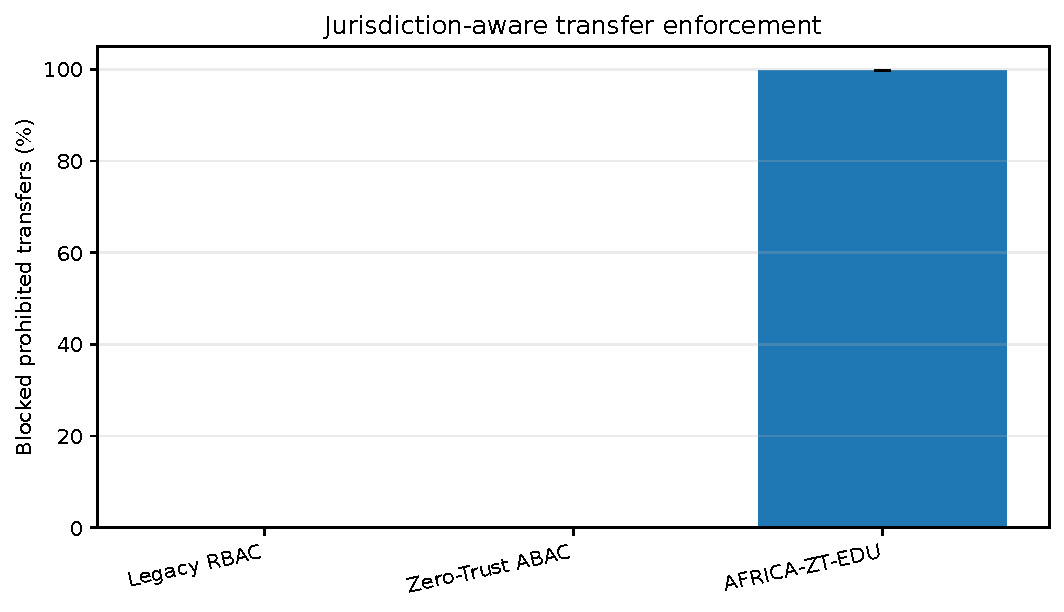
\includegraphics[width=0.49\textwidth]{figures/transfer_blocking.pdf}\label{fig:transferblock}}\\[-0.5ex]
\subfloat[Mean released fields per permitted request.]{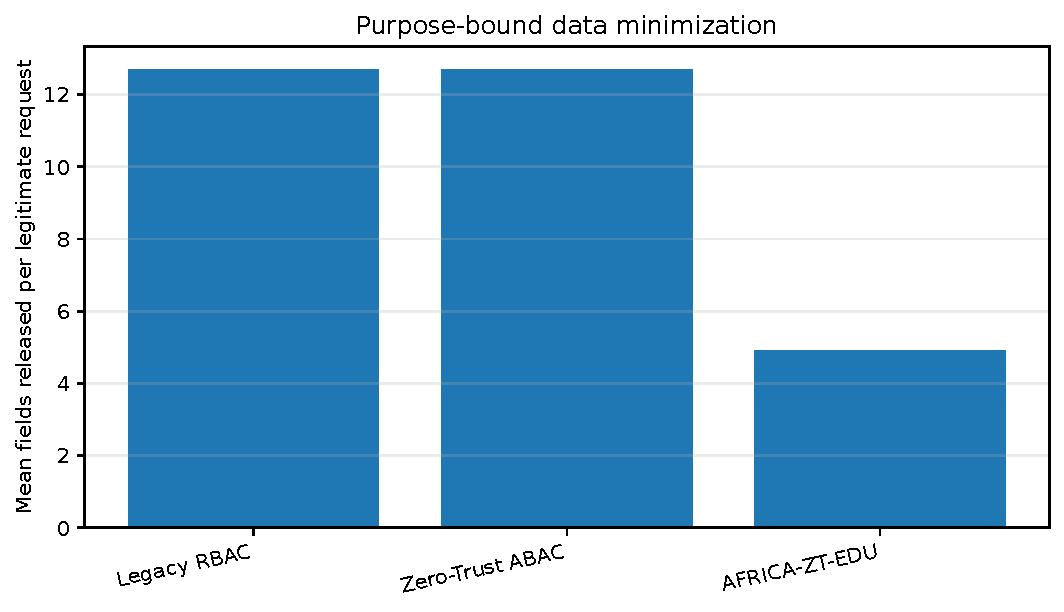
\includegraphics[width=0.49\textwidth]{figures/data_minimization.pdf}\label{fig:minimization}}
\hfill
\subfloat[Modeled in-process policy latency, excluding network RTT.]{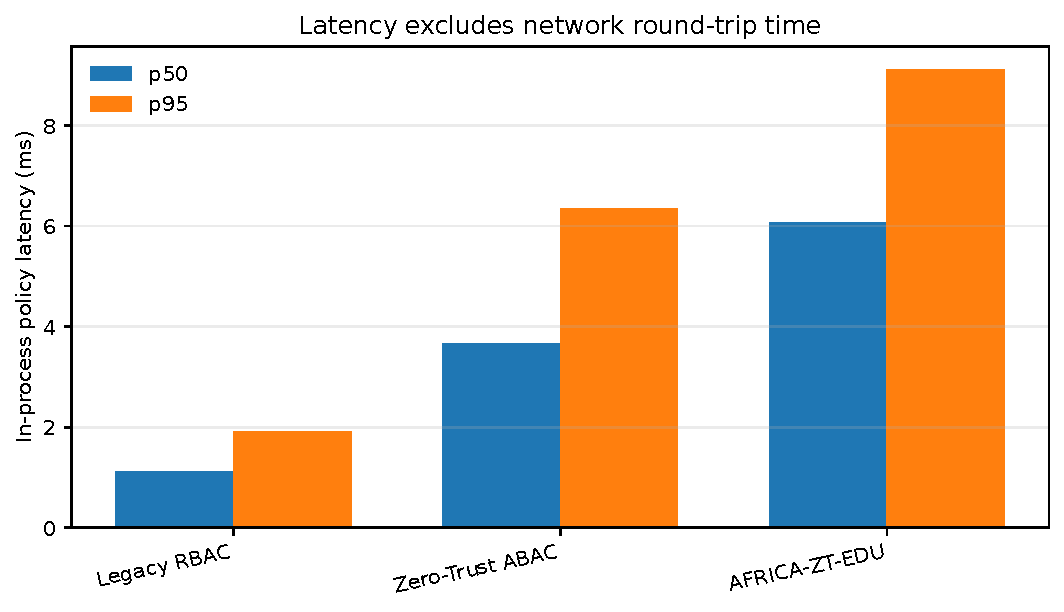
\includegraphics[width=0.49\textwidth]{figures/policy_latency.pdf}\label{fig:modellatency}}
\caption{Synthetic policy-evaluation results. Error bars are 95\% intervals across 30 seeds; the y-axis and scope differ by panel. Latency is generated by the declared simulator and is not the measured microbenchmark reported later.}
\label{fig:policycombined}
\end{figure*}

The results answer RQ3 within the model. Coarse RBAC permits many requests that violate purpose, identity-context, or transfer truth. Contextual ABAC removes a large share of those errors but cannot distinguish an otherwise legitimate request whose purpose, basis, or destination profile makes the release invalid. The full architecture reduces the false-permit rate to 0.0095\%, with the remaining error produced by deliberately stale false-allow registry entries. The 0.104\% legitimate-denial rate is likewise produced by configured stale false-deny entries. Purpose-bound field projection reduces the mean disclosed schema from 12.702 to 4.920 fields, a 61.26\% reduction. These quantities demonstrate generator-level policy expressiveness; they do not imply equivalent reductions in production breaches or legal risk.

\subsection{Registry-Staleness and Differential-Privacy Sensitivity}
Because the jurisdiction registry is a governance dependency, the artifact isolates its failure mode over 200,000 otherwise-valid prohibited-transfer candidates. The observed escape rate tracks the configured stale/incorrect false-allow rate almost linearly. At 0.25\% stale entries, 0.2525\% of prohibited candidates escape; at 1\%, 0.9980\% escape; at 5\%, 5.0045\% escape. This result is intentionally unsurprising: it quantifies why signed updates, review ownership, rollback protection, freshness limits, and fail-closed behavior are architectural requirements rather than administrative details.

The DP utility experiment applies Laplace noise to 50,000 synthetic cohort counts with cohort sizes from 25 to 250. At $\epsilon=1$, the median absolute error is 0.550 percentage points, the mean is 1.018, and the 95th percentile is 3.591. Lower $\epsilon$ improves formal privacy but increases error; higher $\epsilon$ reduces error while weakening the per-query privacy guarantee. Production analytics would additionally require composition accounting, clipping, contribution limits, minimum cohort sizes, repeated-query controls, and leakage testing.

\begin{table*}[t]
\caption{Sensitivity Results for Policy Registry Staleness and Differential Privacy}
\label{tab:sensitivity}
\centering
\scriptsize
\begin{tabularx}{\textwidth}{|C|C|C|C|C|C|}
\hline
\THead{Stale transfer entries \%} & \THead{Prohibited-transfer escape \%} & \THead{Blocked \%} & \THead{$\epsilon$} & \THead{Median abs. error (pp)} & \THead{95th-pctl abs. error (pp)} \\
\hline
0.00 & 0.0000 & 100.0000 & 0.25 & 2.1957 & 14.6139 \\
\hline
0.10 & 0.1010 & 99.8990 & 0.50 & 1.1094 & 7.2606 \\
\hline
0.25 & 0.2525 & 99.7475 & 1.00 & 0.5497 & 3.5913 \\
\hline
0.50 & 0.4870 & 99.5130 & 2.00 & 0.2727 & 1.7944 \\
\hline
1.00 & 0.9980 & 99.0020 & 4.00 & 0.1359 & 0.9254 \\
\hline
2.00 & 1.9715 & 98.0285 & 8.00 & 0.0686 & 0.4567 \\
\hline
5.00 & 5.0045 & 94.9955 & -- & -- & -- \\
\hline
\end{tabularx}
\end{table*}

\begin{figure*}[t]
\centering
\subfloat[Policy-registry staleness.]{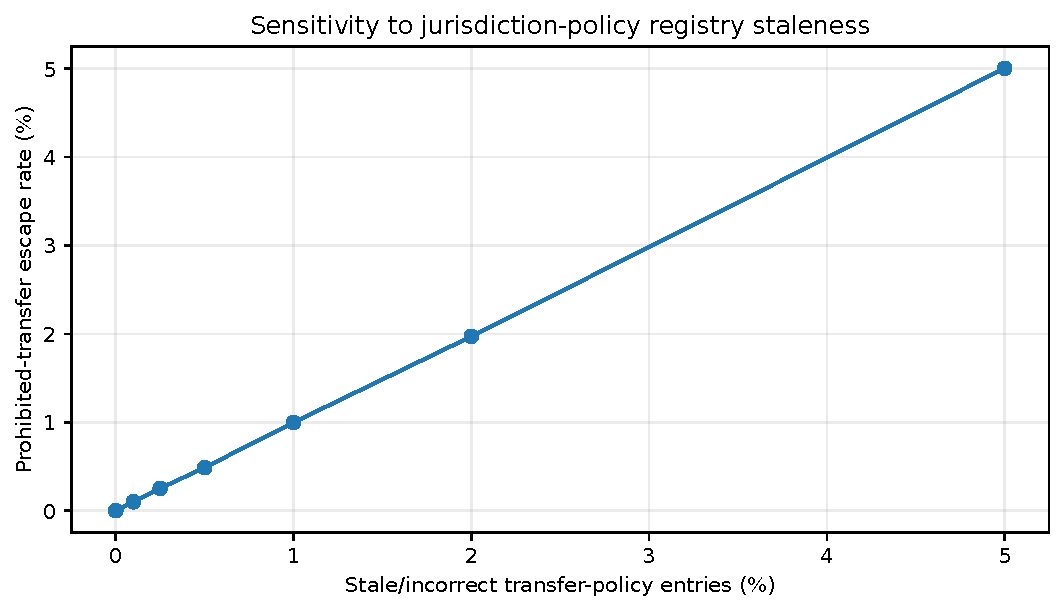
\includegraphics[width=0.49\textwidth]{figures/policy_staleness.pdf}\label{fig:staleness}}
\hfill
\subfloat[Differential-privacy utility.]{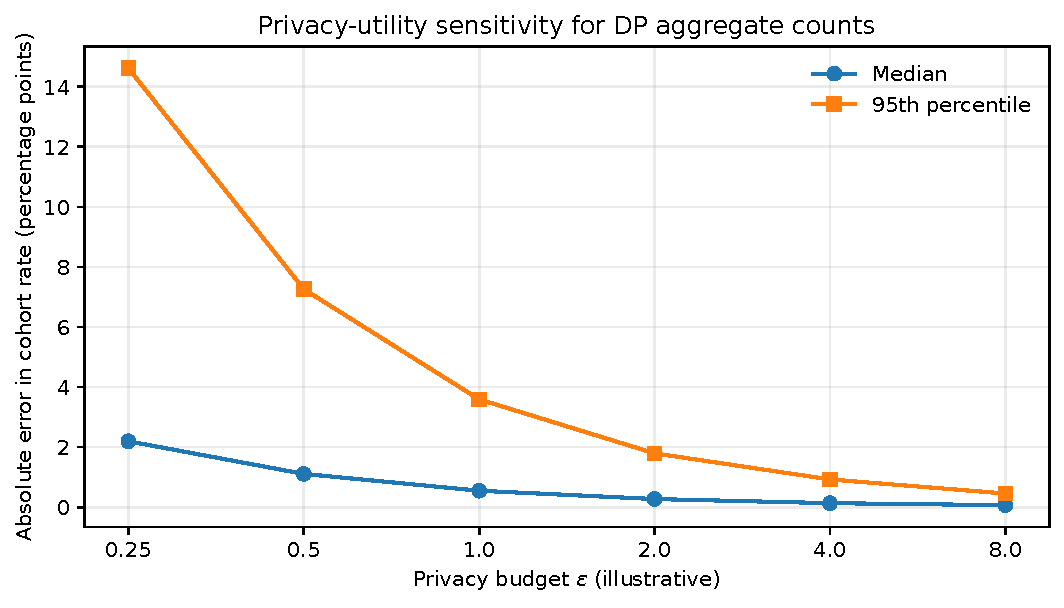
\includegraphics[width=0.49\textwidth]{figures/dp_utility.pdf}\label{fig:dputility}}
\caption{Sensitivity analyses. The left panel isolates incorrect transfer-policy entries; the right panel uses synthetic count queries and reports error in percentage points. Neither panel is a country-level observation.}
\label{fig:sensitivityplots}
\end{figure*}

\subsection{Reproducible Microbenchmark}
The computational demonstration measures operations expected at a policy gateway: Ed25519 signing and verification of a canonical 720-byte VC-like payload; AES-256-GCM encryption and decryption for 1, 10, and 100~KiB buffers; sequential first-match policy evaluation over 50 and 200 rules; and a composite gate containing signature verification, a conservative 200-rule scan with the permit rule placed last, encryption of a 10~KiB payload, and generation of a hashed decision receipt.

The benchmark uses Python 3.13.5, \texttt{cryptography} 46.0.4, and NumPy 2.3.5 on an x86\_64 Linux host. It warms each operation before recording samples and publishes both raw and summary CSV files. All payloads are synthetic. The benchmark excludes network, database, key-management appliance, orchestration, storage, user-interface, and remote identity-provider latency. It therefore estimates local computational cost, not production response time.

\begin{table}[t]
\caption{Selected Single-Host Microbenchmark Results}
\label{tab:benchmark}
\centering
\scriptsize
\begin{tabularx}{\columnwidth}{|Y|p{0.11\columnwidth}|p{0.16\columnwidth}|p{0.16\columnwidth}|}
\hline
\THead{Operation} & \THead{$n$} & \THead{p50 ms} & \THead{p95 ms} \\
\hline
Ed25519 sign, 720 B & 5000 & 0.0326 & 0.0442 \\
\hline
Ed25519 verify, 720 B & 5000 & 0.1028 & 0.1231 \\
\hline
AES-GCM encrypt, 10 KiB & 3000 & 0.0019 & 0.0021 \\
\hline
Policy scan, 50 rules & 6000 & 0.0016 & 0.0016 \\
\hline
Policy scan, 200 rules & 4000 & 0.0048 & 0.0052 \\
\hline
Composite authorization gate & 2500 & 0.1210 & 0.1384 \\
\hline
\end{tabularx}
\end{table}

\begin{figure*}[t]
  \centering
  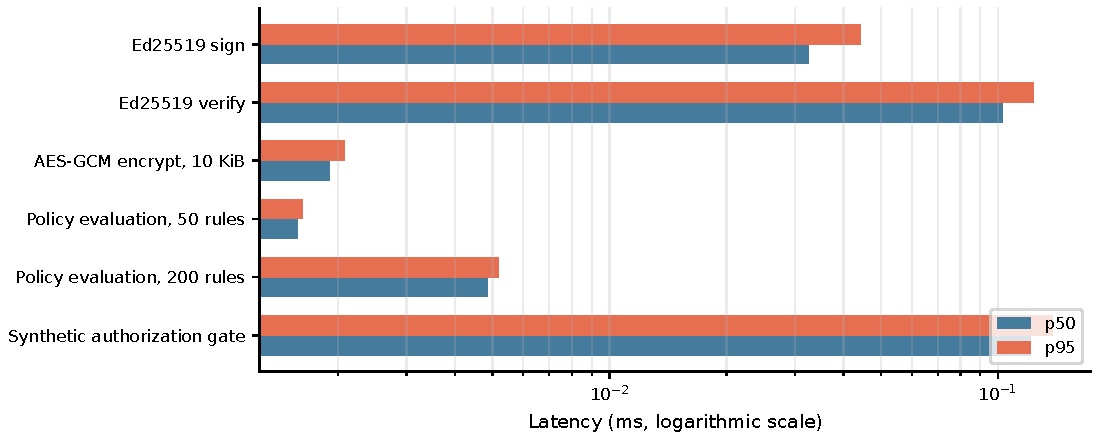
\includegraphics[width=0.90\textwidth]{figures/benchmark_latency.pdf}
  \caption{Median and 95th-percentile latency for selected synthetic operations. The logarithmic horizontal axis exposes both cryptographic verification and lower-latency policy/encryption operations.}
  \label{fig:benchmark}
\end{figure*}

Ed25519 verification is the largest measured component of the composite path. Increasing the conservative sequential rule set from 50 to 200 raises median policy latency from 0.0016 to 0.0048~ms, consistent with a near-linear scan at this scale. The composite gate records 0.1210~ms median and 0.1384~ms p95. These results indicate that the local policy and cryptographic operations need not dominate a typical Internet-mediated educational request. They do not establish performance on mobile devices, hardware security modules, congested networks, multi-region databases, or production policy engines.

\section{Discussion}
\subsection{RQ1: Requirements Are Joint, Not Sequential}
The evidence synthesis shows that cross-border educational architecture cannot be designed as ``security first, compliance later.'' Identity assurance, purpose limitation, minimization, transfer conditions, learner rights, credential integrity, accountability, and resilience interact. A passkey can reduce account takeover but does not justify exporting an entire learner profile. A signed credential can establish origin and integrity but does not establish academic quality or recognition. A local data region can support control over authoritative records but does not prove that a processing purpose is necessary. R1--R14 therefore form a coupled control system rather than an optional checklist.

The context indicators also caution against claims of continental uniformity. A broad trend toward privacy legislation coexists with different transfer rules, regulator procedures, institutional capacities, and treaty participation. The appropriate technical response is a shared control vocabulary with reviewed institution- and jurisdiction-specific profiles, not a lowest-common-denominator rule and not 55 unrelated application designs.

\subsection{RQ2: A Policy-Gated Claim Architecture}
The central design choice is to combine zero-trust authorization with privacy and transfer obligations. Conventional ABAC asks whether a subject may perform an action on a resource. The proposed PDP additionally asks why the action is needed, which recipient and destination are involved, which data category is requested, which basis or safeguard has been approved, which fields are proportionate, how long the view should live, and what evidence must be retained. The output is therefore a short-lived minimized claim view plus enforceable obligations and a signed receipt.

This pattern avoids two extremes. Blanket localization can fragment course collaboration and credential recognition, while unrestricted replication exposes complete records to unnecessary institutions, jurisdictions, and vendors. Regional authoritative zones with controlled claim exchange preserve interoperability without assuming that every service should store the source database. The same pattern can support course consortia, credit transfer, joint programs, professional credentials, employer verification, and regulator review.

\subsection{RQ3: Policy Expressiveness, Minimization, and Registry Quality}
Within the declared generator, purpose, basis, jurisdiction, and field-projection predicates materially change decision quality. Zero-trust ABAC reduces the false-permit rate relative to coarse RBAC, but it still lacks the information needed to reject an otherwise context-valid prohibited transfer. The proposed architecture's remaining false permits and legitimate denials are driven by deliberately injected registry staleness. Consequently, the strong result should not be read as a generic algorithmic guarantee: it demonstrates that the richer model can express the synthetic ground truth when its policy data are current.

The minimization result is equally important. The architecture releases an average of 4.920 fields rather than 12.702, reducing the disclosure surface by 61.26\% for permitted synthetic requests. This metric does not prove that the selected fields are legally minimal in a real case. It shows that field projection can be made explicit, testable, and measurable instead of being left to application developers.

\subsection{RQ4: Coverage, Local Cost, and Privacy Utility}
The 34/36 analytical score improves because controls are explicit and cross-linked rather than isolated. The strongest gains occur for token replay, compromised devices, governed transfer, credential status, and evidence integrity. Full scores are intentionally withheld for analytics leakage, connectivity, and semantic policy error. A 100\% score would conceal irreducible and organizational risks.

The microbenchmark supports a narrower performance conclusion: selected local cryptographic and policy operations are computationally modest on the recorded host. It cannot establish end-to-end service-level objectives. Production pilots must measure remote identity-provider latency, database/cache behavior, hardware-backed keys, policy distribution, mobile-wallet verification, packet loss, regional failover, and audit ingestion. Similarly, the DP study shows a tunable utility trade-off for synthetic counts, not that every learning-analytics task should or can use the same mechanism.

\subsection{Deployment Roadmap}
A staged deployment reduces both security and institutional risk. Each phase should include accessibility, language, low-bandwidth, and usability testing, because a cryptographically strong workflow that learners cannot understand can shift risk to shared accounts, unsafe recovery, help-desk impersonation, and exclusion.

\begin{table*}[t]
\caption{Three-Phase Implementation and Assurance Roadmap}
\label{tab:roadmap}
\centering
\footnotesize
\begin{tabularx}{\textwidth}{|p{0.13\textwidth}|p{0.18\textwidth}|p{0.34\textwidth}|Y|}
\hline
\THead{Phase} & \THead{Indicative horizon} & \THead{Core engineering and governance work} & \THead{Exit evidence} \\
\hline
1. Institutional foundation & 0--6 months & Inventory data/flows; classify resources; separate workload identities; deploy phishing-resistant access for privileged roles; centralize PDP/PEP; define purpose, retention, rights, incident, and key-management ownership. & Approved data-flow register; privileged-access test; deny-path suite; key-rotation drill; high-risk decision receipts; baseline accessibility and recovery test. \\
\hline
2. Governed federation & 6--18 months & Establish partner and issuer trust registries; encode reviewed jurisdiction profiles; deploy transfer gateway; introduce minimized views and interoperable credentials; test status, revocation, partner exit, and cross-institution incident coordination. & Signed partner profiles; transfer-policy conformance tests; blocked-transfer evidence; credential interoperability test; revocation propagation; exit/migration rehearsal. \\
\hline
3. Privacy-enhanced analytics & 18--36 months & Separate operational and analytical stores; introduce pseudonymization, cohort floors, budgets, secure aggregation or federated computation; publish learner explanations; evaluate benefit, bias, and model leakage. & Privacy-budget ledger; small-cohort denial; repeated-query test; utility and leakage report; learner-facing transparency review; independent security/privacy assessment. \\
\hline
\end{tabularx}
\end{table*}

\subsection{Governance and Assurance}
The architecture requires governance artifacts alongside code: a data and purpose catalog; jurisdiction-profile ownership; key-management policy; issuer onboarding criteria; credential schema governance; revocation authority; privacy-impact and transfer-assessment templates; rights and appeal workflows; incident roles; change approval; and vendor-exit plans. Signed receipts make decisions reviewable, but competent review bodies must exist and have authority. Open standards reduce lock-in only when contracts preserve data export, key control, documentation, and transition assistance.

Assurance should be evidence-based rather than brand-based. Recommended evidence includes policy unit and property tests, deny-path tests, key-rotation drills, status-list freshness tests, simulated rights requests, transfer-register reconciliation, configuration-drift scans, restore exercises, accessibility and language tests, and independent penetration testing. Higher-risk proctoring and analytics additionally require necessity, proportionality, bias, and non-digital-alternative review.

\section{Limitations, Validity Threats, and Future Work}
\subsection{Construct and Internal Validity}
The analytical score depends on the declared comparator, objective definitions, and 0/0.5/1 rubric. It measures explicit control presence, not exploit resistance, operational maturity, or administrator behavior. Independent reviewers may assign different scores. The synthetic policy experiment uses a ground truth generated from the same conceptual predicates used to motivate the architecture, creating a favorable construct alignment. The comparison remains useful for exposing incremental expressiveness, but it cannot prove real-world superiority. Publishing row-level scores, per-seed metrics, and generator code permits sensitivity analysis and replacement of the baseline.

The simulator's latency is modeled rather than measured. It is retained to compare path complexity under a fixed distribution and is clearly separated from the single-host microbenchmark. The microbenchmark itself omits network, storage, parsing, distributed consistency, cold starts, hardware-security modules, mobile hardware, and multi-tenant contention. Timing values must not be transferred to production capacity planning without new measurement.

\subsection{External, Legal, and Organizational Validity}
No real country, institution, learner, regulator, or cloud deployment is evaluated. The legal discussion is purposive and illustrative; it does not enumerate every African law, sector rule, regulator decision, localization requirement, treaty update, or contractual regime. Every jurisdiction profile requires current review by competent institutional and legal personnel. The architecture is law-aware but not law-determining and does not certify a transfer.

The connectivity and governance indicators are aggregate contextual signals with different denominators and dates. They do not characterize every locality, institution, or learner. Organizational capability, procurement constraints, legacy integration, staffing, language, accessibility, and trust relationships may dominate technical feasibility. No human-subject study evaluates learner comprehension, consent quality, recovery burden, perceived surveillance, disability access, or institutional cost.

\subsection{Privacy and Security Residual Risk}
Zero trust reduces implicit trust but does not eliminate compromised endpoints, malicious insiders, supply-chain compromise, coerced users, fraudulent issuers, semantic policy mistakes, or insecure recovery. Verifiable credentials prove issuer-controlled statements and integrity; they do not prove educational quality or legal recognition. Differential privacy and federated analytics reduce selected disclosure risks but do not make models or repeated analyses risk-free. Offline acceptance necessarily creates bounded freshness risk.

\subsection{Future Work}
Future work should implement a standards-conformant prototype with a production policy engine, workload identity, hardware-backed keys, credential-wallet interoperability, proof-bound tokens, and a formal jurisdiction-profile schema. Multi-country pilots should test low-bandwidth synchronization, status under intermittent connectivity, rights workflows, incident coordination, regulator-facing evidence, and partner exit. Red-team exercises should include token replay, compromised issuer keys, malicious partner APIs, slow exfiltration, policy rollback, recovery abuse, registry poisoning, and analytics inference. Participatory research with learners, educators, registrars, disability advocates, privacy professionals, and regulators should determine whether the system delivers understandable agency rather than technical compliance alone.

\section{Ethics, Data, and Reproducibility Statement}
The study uses only synthetic requests, synthetic cohort counts, abstract jurisdiction profiles, and local cryptographic test payloads. It contains no human-subject interaction, personal data, biometric sample, student record, production institution log, or named-country policy performance result. The companion artifact includes the complete \LaTeX{} source, Bib\TeX{} database, source CSV files, per-seed metrics, raw benchmark measurements, environment metadata, vector/raster figures, and scripts for regenerating the policy simulation, DP study, staleness study, microbenchmark, and figures. A public archival DOI or repository URL should be inserted only after the author deposits the final reviewed artifact.

The author declares that the architecture and experiments are research artifacts and do not constitute legal advice, accreditation evidence, vendor certification, or a guarantee of security. No external funding source or conflict of interest is declared in this article.

\section{Conclusion}
This paper presents \system, a policy-centric zero-trust and privacy-preserving reference architecture for cross-border digital education in Africa. Its central claim is architectural: protected-data decisions should bind subject, device, workload, resource, action, purpose, basis, jurisdiction, minimization, risk, and accountability before a receiving service obtains learner data. Regional encrypted zones retain authoritative records; transfer gateways release short-lived claim views; W3C Verifiable Credentials support portable academic proof; privacy-enhanced analytics reduce unnecessary pooling; and signed receipts make decisions reviewable.

The design derives fourteen traceable requirements, reaches 34 of 36 analytical control objectives under a declared rubric, and is evaluated over 3,000,000 synthetic requests. Under those assumptions, it records a 0.0095\% false-permit rate, blocks 99.750\% of otherwise-authorized prohibited transfers, and reduces average disclosed fields by 61.26\%. A separate local microbenchmark records 0.1210~ms median and 0.1384~ms p95 for the selected composite gate, while the DP experiment demonstrates an explicit privacy-utility trade-off. These results are encouraging but deliberately bounded. Deployment quality will depend on current legal review, policy-data quality, institutional governance, usable recovery, key management, low-connectivity engineering, accessibility, and independent security/privacy validation. The included artifact makes the assumptions, data, figures, and measurements inspectable so that subsequent studies can challenge the model and extend it through real pilots.

\section*{Artifact Availability}
The Overleaf-ready companion package includes the complete article source, bibliography, fully bordered table design, vector and raster figures, contextual source data, row-level threat scores, 30-seed policy results, DP and staleness outputs, raw microbenchmark samples, environment metadata, and executable scripts. A public archival repository identifier should be added before journal submission.

\balance
\bibliographystyle{IEEEtran}
\bibliography{references}

\end{document}
